\section{Introdução ao LibreOffice Impress}

\begin{frame}{}
	\begin{block}{}
		\begin{itemize}
			\item O Impress é o programa de \textbf{apresentações} incluído no LibreOffice.
			\item Você pode criar slides que contenham vários elementos diferentes, incluindo \textbf{texto}, \textbf{listas com marcadores}, \textbf{numeração}, \textbf{tabelas}, \textbf{gráficos} e etc.
			\item O Impress inclui também um \textbf{verificador ortográfico}, um \textbf{dicionário de sinônimos}, \textbf{estilos de texto}, e \textbf{estilos de plano de fundo}.
		\end{itemize}
	\end{block}

	\medskip

	\centering
	
\includegraphics[width=0.3\linewidth]{Figuras/Ch05/fig1}
\end{frame}


\begin{frame}{}
	
	\centering
	
\includegraphics[width=1\linewidth]{Figuras/Ch05/fig0.1}
\end{frame}


\begin{frame}{Criando um aquivo do Impress}
	\begin{block}{}
		\begin{itemize}
			\item Você pode iniciar o Impress de \textbf{várias formas}, como o Writer.
			\item Quando você iniciar o Impress, a janela principal é exibida.
		\end{itemize}
	\end{block}

	\centering
	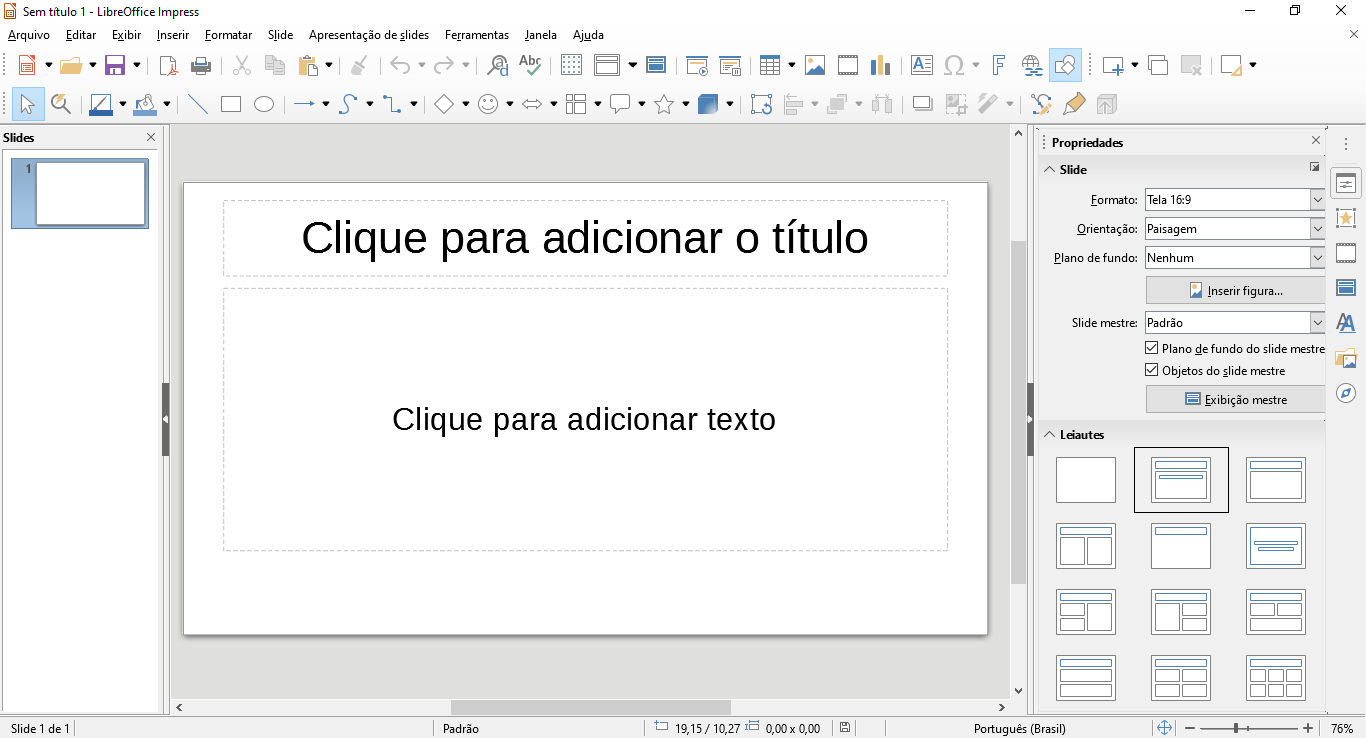
\includegraphics[width=0.8\linewidth]{Figuras/Ch05/fig2}
\end{frame}


\begin{frame}{Janela principal do Impress}
	\begin{block}{}
		A janela principal do Impress tem três partes:
		\begin{enumerate}
			\item painel de slides;
			\item área de trabalho;
			\item painel lateral.
		\end{enumerate}
		Além disso, várias \textbf{barras de ferramentas} podem ser \textbf{exibidas} ou \textbf{ocultadas} durante a criação de uma apresentação.
	\end{block}

	\centering
	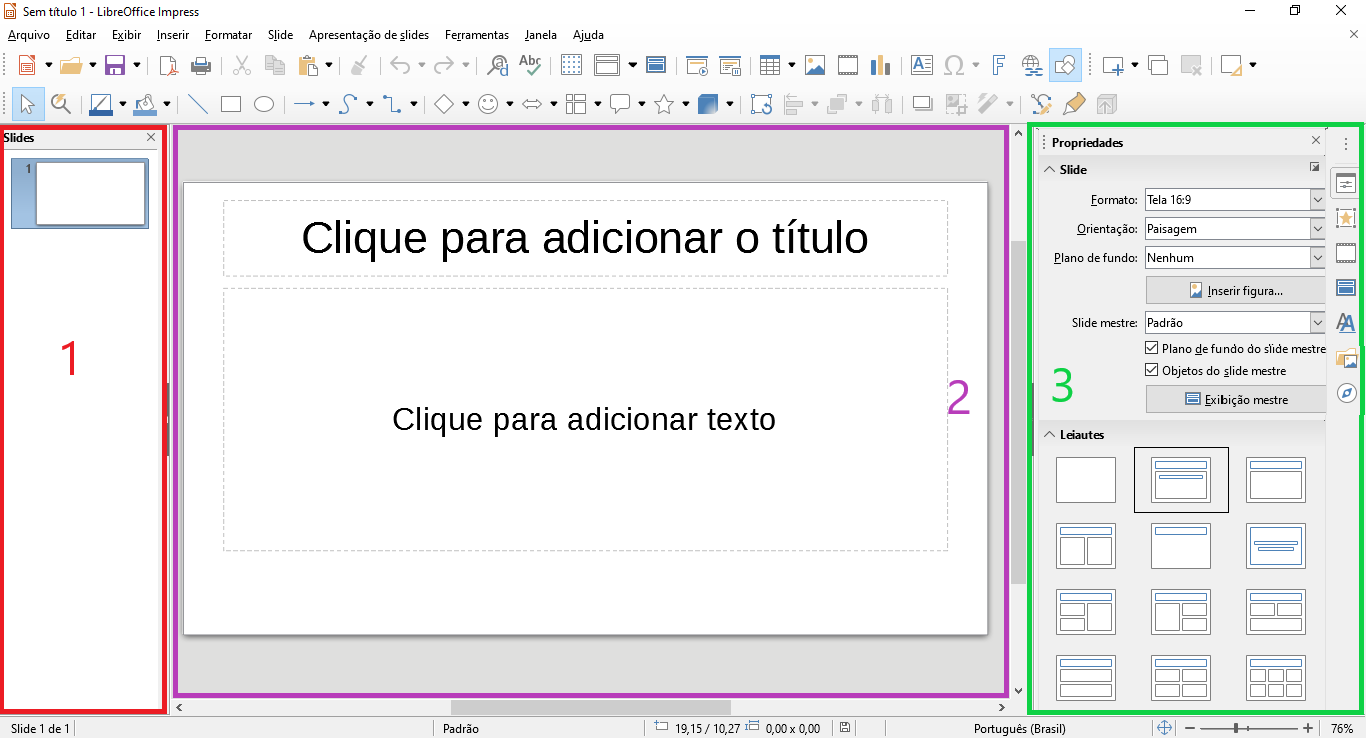
\includegraphics[width=0.6\linewidth]{Figuras/Ch05/fig3}
\end{frame}


\begin{frame}{Janela principal do Impress}
	\begin{block}{}
		\begin{itemize}
			\item A exibição ou não das partes da Janela Principal do Impress é uma questão de \textbf{preferência} do usuário.
			\item Você pode fechar o Painel de slides ou o Painel lateral, clicando no \textbf{X} no \textbf{canto superior direito} do painel, ou ir em Exibir > Painel de slides ou Exibir > Barra lateral na barra de menu principal para \textbf{desmarcar} o painel.
		\end{itemize}
	\end{block}

	\begin{minipage}{0.49\linewidth}
		\centering
		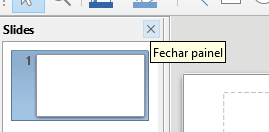
\includegraphics[width=1\linewidth]{Figuras/Ch05/fig4}
	\end{minipage}\hfill
	\begin{minipage}{0.49\linewidth}
		\centering
		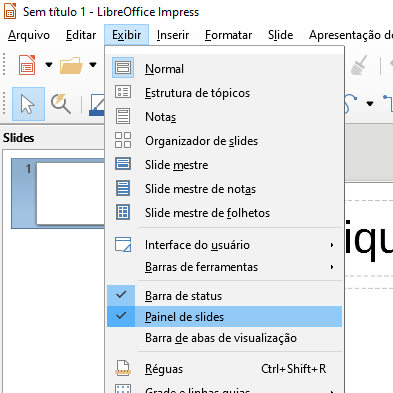
\includegraphics[width=0.75\linewidth]{Figuras/Ch05/fig5}
	\end{minipage}
\end{frame}


\begin{frame}{Janela principal do Impress}
	\begin{block}{}
		\begin{itemize}
			\item Você também pode \textbf{maximizar} a Área de trabalho clicando no \textbf{marcador} Ocultar/Mostrar no meio da linha de separação vertical.
			\item Usar o marcador Ocultar/Mostrar \textbf{esconde}, mas \textbf{não fecha}, os painéis de Slides e Tarefas.
		\end{itemize}
	\end{block}

	\centering
	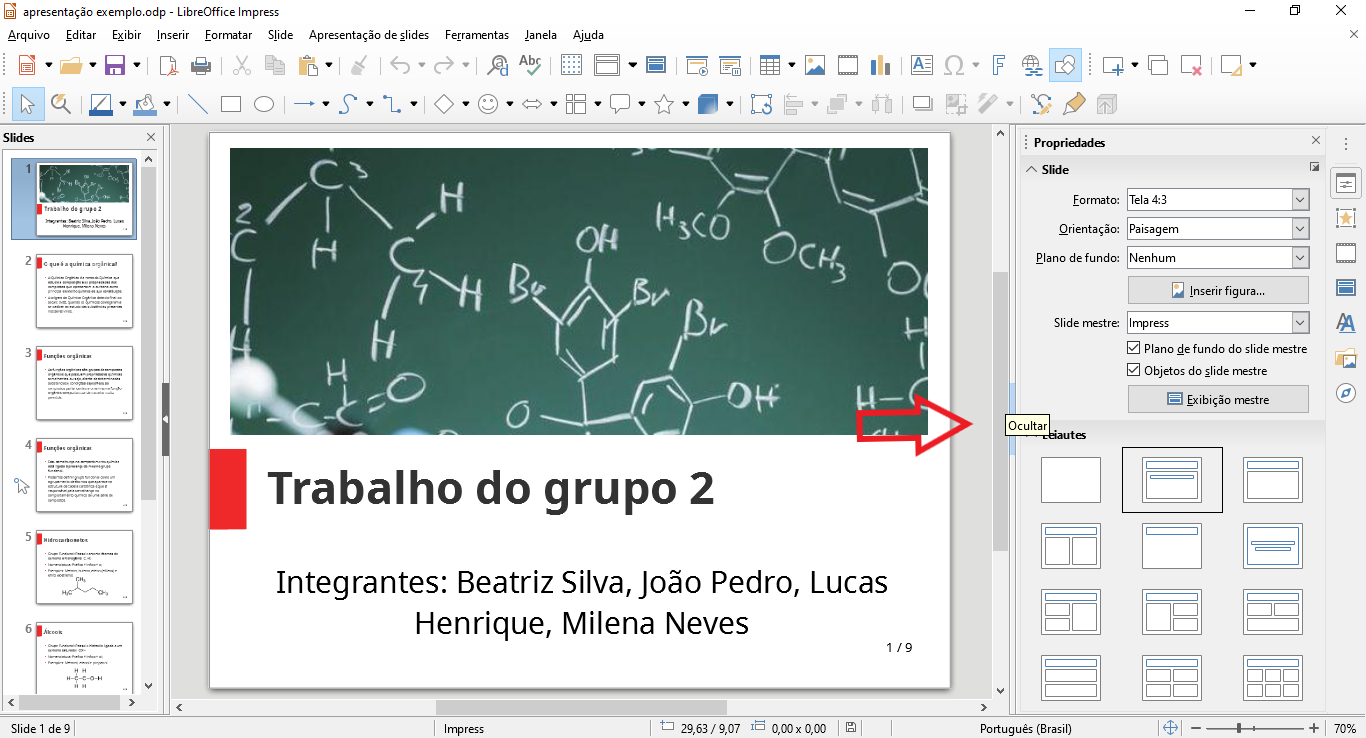
\includegraphics[width=0.8\linewidth]{Figuras/Ch05/fig6}
\end{frame}


\begin{frame}{Janela principal do Impress}
	\begin{block}{}
		\begin{itemize}
			\item Para \textbf{restaurar} o painel, clique \textbf{novamente} em seu marcador Ocultar/Mostrar.
		\end{itemize}
	\end{block}
	
	\centering
	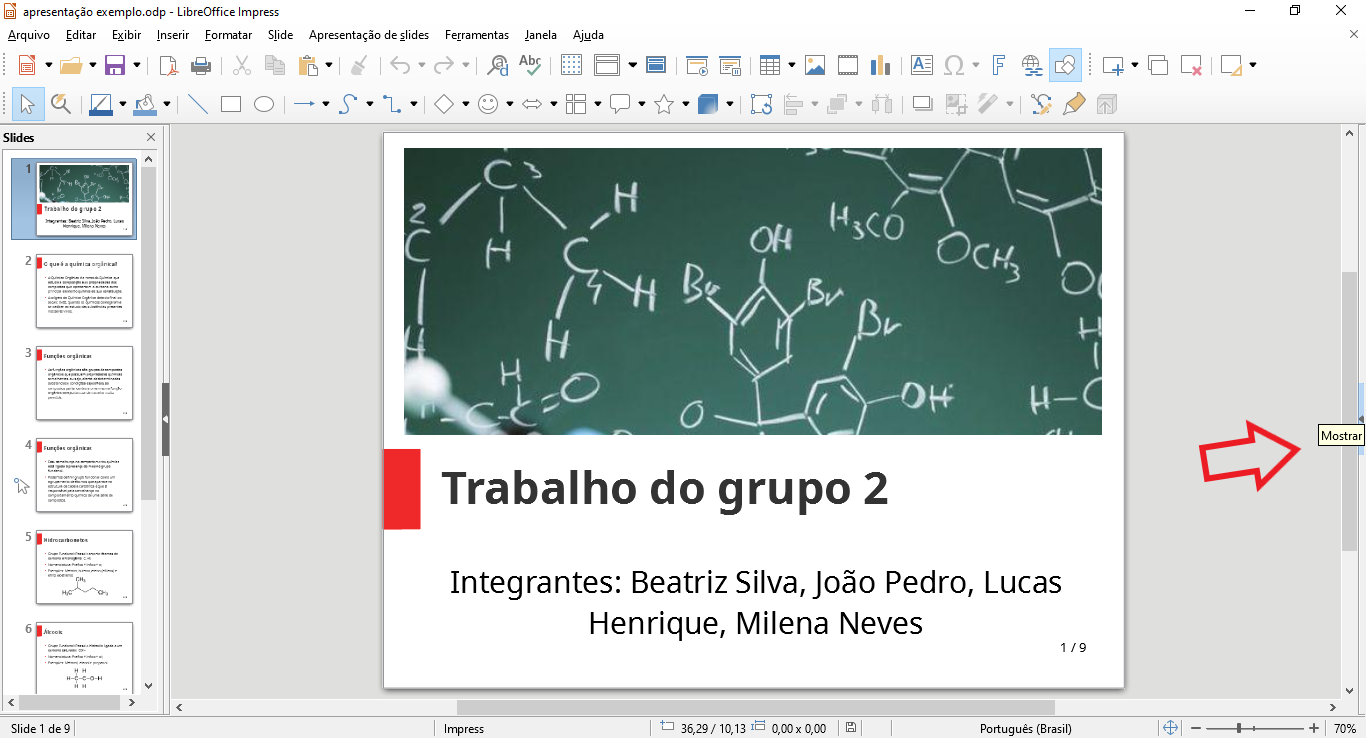
\includegraphics[width=0.9\linewidth]{Figuras/Ch05/fig7}
\end{frame}


\begin{frame}{Painel de slides}
	\begin{block}{}
		\begin{itemize}
			\item O Painel de slides contém imagens em \textbf{miniatura} dos slides em sua apresentação, na ordem em que serão mostradas.
			\item Clicando em um slide neste painel, este é selecionado e colocado na \textbf{Área de trabalho}.
			\item Quando um slide está na Área de trabalho, você pode \textbf{fazer alterações }nele.
		\end{itemize}
	\end{block}

	\centering
	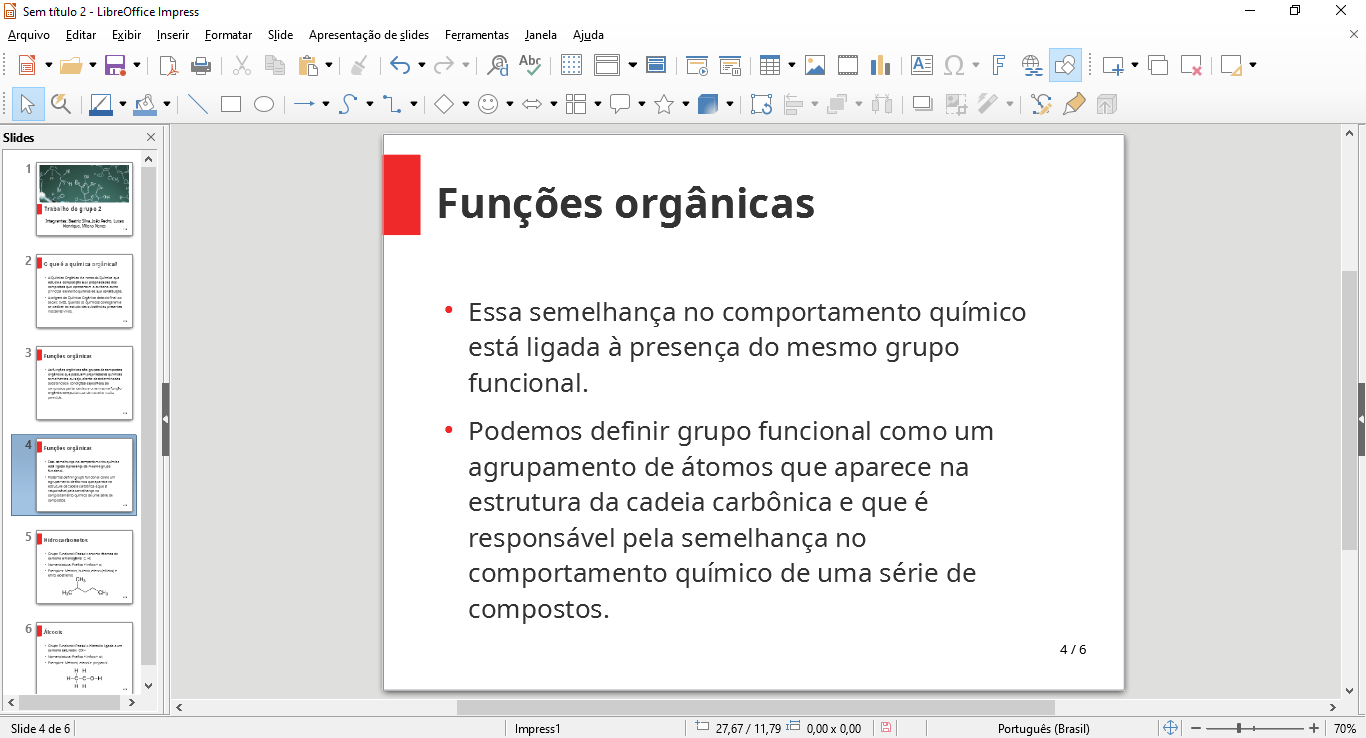
\includegraphics[width=0.7\linewidth]{Figuras/Ch05/fig8}
\end{frame}


\begin{frame}{Painel de slides}
	\begin{block}{Funções principais}
		Várias \textbf{operações adicionais} podem ser realizadas em \textbf{um ou mais} slides \textbf{simultaneamente} no Painel de slides:
		\begin{itemize}
			\item adicionar \textbf{novos slides} para a apresentação;
			\item marcar um slide como \textbf{oculto} para que ele \textbf{não seja exibido} como parte da apresentação;
			\item \textbf{excluir} um slide da apresentação se ele não for mais necessário;
			\item \textbf{renomear} um slide;
			\item \textbf{duplicar} um slide.
		\end{itemize}
	\end{block}
\end{frame}


\begin{frame}{Painel de slides}
	\begin{block}{Outras funções}
		Também é possível realizar as seguintes operações, embora existam métodos mais eficientes do que usar o Painel de slides:
		\begin{itemize}
			\item \textbf{alterar a transição} de slides seguindo o slide selecionado ou após cada slide em um grupo de slides;
			\item \textbf{alterar o design} de slide;
			\item \textbf{alterar o layout} de slide para um grupo de slides simultaneamente.
		\end{itemize}
	\end{block}
\end{frame}


\begin{frame}{Barra lateral}
	\begin{block}{}
		\begin{itemize}
			\item A Barra lateral tem \textbf{sete seções}.
			\item Para expandir uma seção que você deseja usar, clique no \textbf{ícone}.
			\item Somente \textbf{uma seção} pode ser aberta de cada vez.
		\end{itemize}
	\end{block}

	\centering
	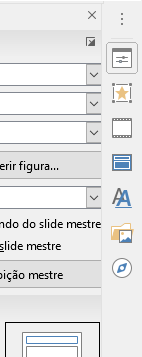
\includegraphics[width=0.19\linewidth]{Figuras/Ch05/fig9}
\end{frame}


\begin{frame}{Barra lateral}
	\begin{block}{Propriedades}
		\begin{itemize}
			\item Mostra os \textbf{leiautes} (\textit{layouts}) incluídos no Impress.
			\item Você pode escolher algum e usá-lo \textbf{como ele é}, ou \textbf{modificá-lo} para atender às suas necessidades.
			\item No entanto, não é possível salvar \textbf{leiautes personalizados}.
		\end{itemize}
	\end{block}

	\centering
	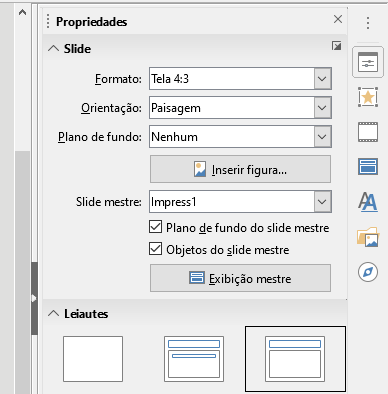
\includegraphics[width=0.4\linewidth]{Figuras/Ch05/fig9.1}
\end{frame}


\begin{frame}{Barra lateral}
	\begin{block}{Transição de slides}
		\begin{itemize}
			\item Fornece acesso a um número de opções de \textbf{transição de slides}.
			\item O padrão é definido como \textbf{Sem transição}, em que o slide seguinte \textbf{substitui} o existente.
			\item No entanto, muitas transições adicionais estão disponíveis.
			\item Você também pode \textbf{especificar} a \textbf{velocidade de transição} (Lenta, Média, Rápida), escolher entre uma transição \textbf{automática} ou \textbf{manual}, e escolher \textbf{quanto tempo} o slide selecionado será mostrado (no caso de transição automática).
		\end{itemize}
	\end{block}
\end{frame}


\begin{frame}{Barra lateral}

	\centering
	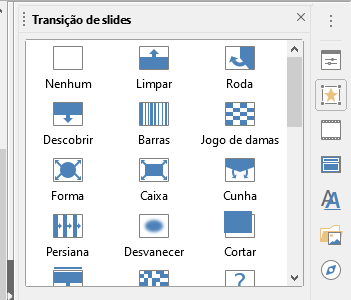
\includegraphics[width=0.75\linewidth]{Figuras/Ch05/fig10}
\end{frame}


\begin{frame}{Barra lateral}
	\begin{block}{Animação}
		\begin{itemize}
			\item Uma variedade de \textbf{animações} podem ser usadas para \textbf{realçar} ou \textbf{melhorar} diferentes elementos de cada slide.
			\item A seção Animação fornece uma maneira fácil para \textbf{adicionar}, \textbf{alterar}, ou \textbf{remover animações}.
		\end{itemize}
	\end{block}

	\centering
	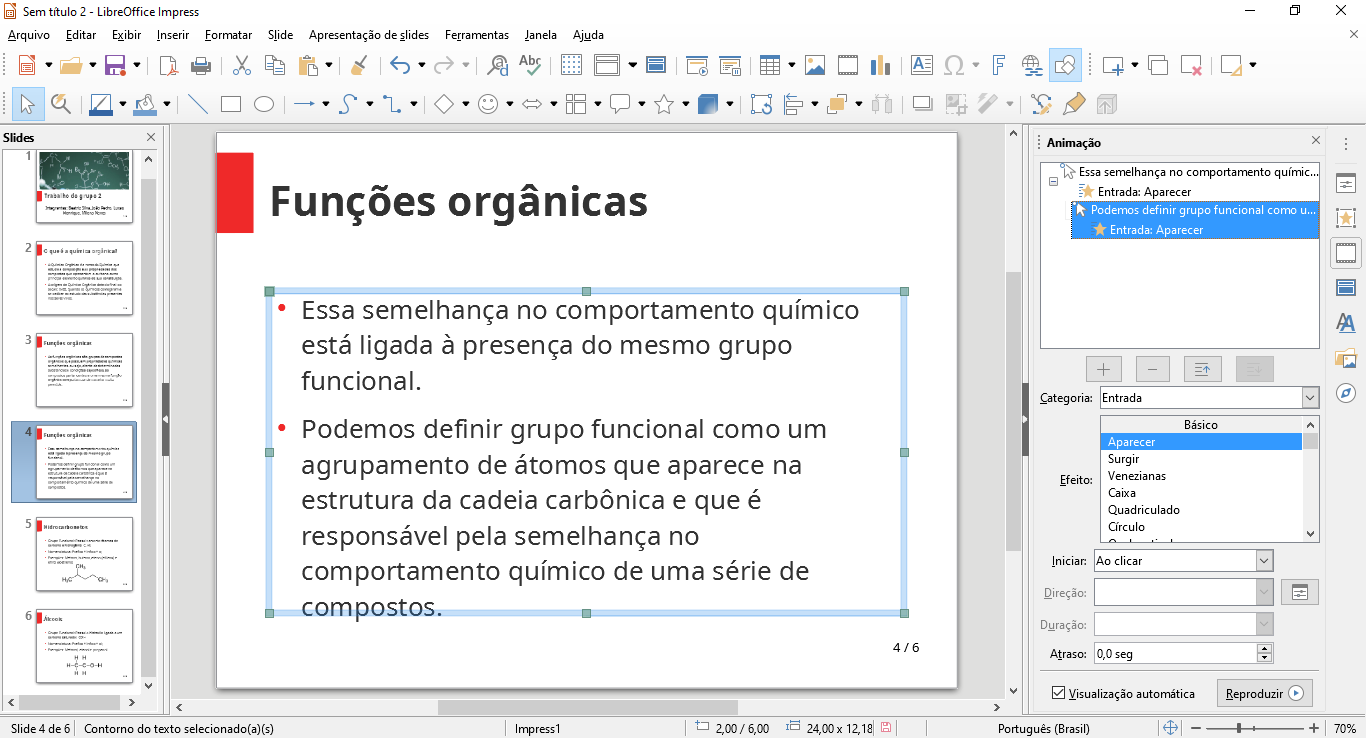
\includegraphics[width=0.75\linewidth]{Figuras/Ch05/fig11}
\end{frame}


\begin{frame}{Barra lateral}
	\begin{block}{Slide mestre}
		\begin{itemize}
			\item Aqui você define o \textbf{estilo de página} (slide) para sua apresentação.
			\item O Impress inclui vários \textbf{modelos} de \textbf{páginas mestras} (\textbf{slide mestre}).
			\item Um deles --- Padrão --- é branco, e o restante tem um \textbf{plano de fundo} e \textbf{estilo de texto}.
		\end{itemize}
	\end{block}

	\centering
	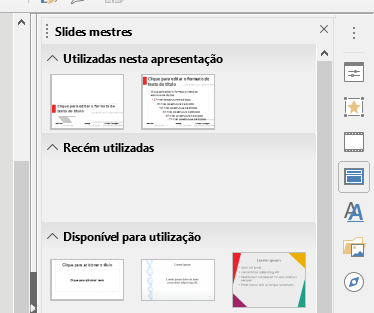
\includegraphics[width=0.48\linewidth]{Figuras/Ch05/fig12}
\end{frame}


\begin{frame}{Barra lateral}
	\begin{block}{Estilos}
		\begin{itemize}
			\item Aqui você pode \textbf{editar} e \textbf{aplicar estilos gráficos} e \textbf{criar estilos novos}.
			\item Quando você edita um estilo, as alterações são \textbf{aplicadas automaticamente} a \textbf{todos} os elementos formatados com este estilo em sua apresentação.
		\end{itemize}
	\end{block}

	\centering
	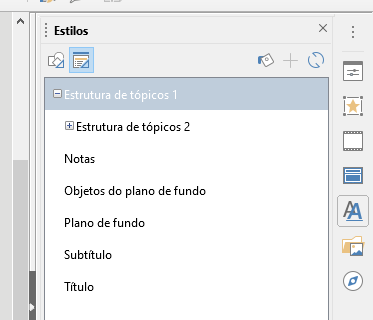
\includegraphics[width=0.43\linewidth]{Figuras/Ch05/fig13}
\end{frame}


\begin{frame}{Barra lateral}
	\begin{block}{Galeria}
		\begin{itemize}
			\item Aqui você pode inserir um \textbf{objeto} em sua apresentação, quer seja como uma \textbf{cópia} ou como um \textbf{link}.
			\item Uma cópia de um objeto é \textbf{independente} do objeto \textbf{original}.
		\end{itemize}
	\end{block}

	\centering
	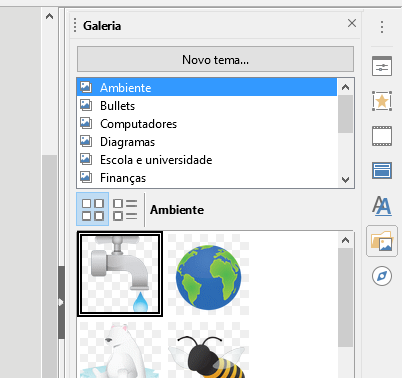
\includegraphics[width=0.45\linewidth]{Figuras/Ch05/fig14}
\end{frame}


\begin{frame}{Barra lateral}
	\begin{block}{Navegador}
		\begin{itemize}
			\item Aqui você pode trabalhar mais facilmente com objetos e a estrutura da apresentação.
			\item Recomenda-se dar \textbf{nomes significativos} aos \textbf{slides} e \textbf{objetos} em sua apresentação para que você possa \textbf{identificá-los} facilmente quando utilizar a navegação.
		\end{itemize}
	\end{block}

	\centering
	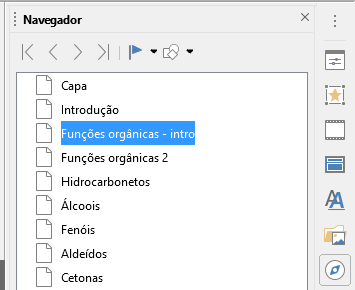
\includegraphics[width=0.4\linewidth]{Figuras/Ch05/fig15}
\end{frame}


\begin{frame}{Alterar formato (tamanho) do slide}
	\begin{block}{Opções de alteração}
		\begin{itemize}
			\item Disponíveis na seção “Propriedades” da Barra lateral, ou;
			\item clicando com o botão direito na área de trabalho e depois, clicar em “Propriedades”.
		\end{itemize}
	\end{block}

	\begin{minipage}{0.49\linewidth}
		\centering
		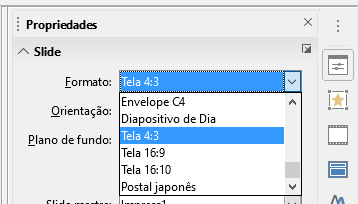
\includegraphics[width=1\linewidth]{Figuras/Ch05/fig16}
	\end{minipage}\hfill
	\begin{minipage}{0.49\linewidth}
		\centering
		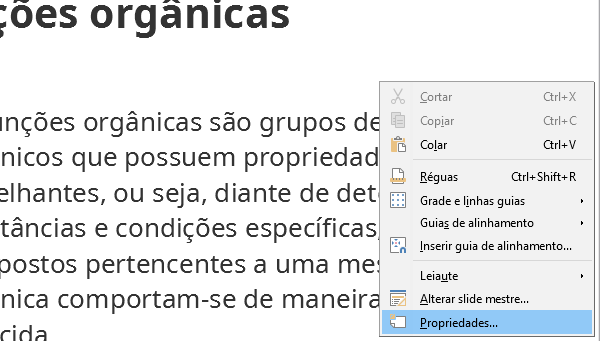
\includegraphics[width=1\linewidth]{Figuras/Ch05/fig16.1}
	\end{minipage}
\end{frame}


\begin{frame}{Alterar formato (tamanho) do slide}
	\begin{block}{Opções de alteração}
		\begin{itemize}
			\item Clicando na barra de menu, clique Slide > Propriedades.
		\end{itemize}
	\end{block}

	\centering
	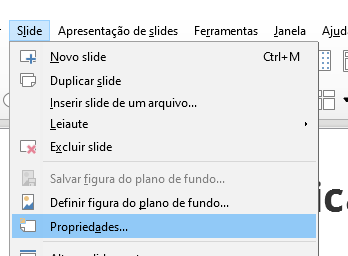
\includegraphics[width=0.7\linewidth]{Figuras/Ch05/fig16.2}
\end{frame}


\begin{frame}{Alterar formato (tamanho) do slide}
	\begin{block}{Opções de alteração}
		\begin{itemize}
			\item Padrão atual $ \to $ 16:9 Padrão anterior $ \to $ 4:3.
		\end{itemize}
	\end{block}

	\centering
	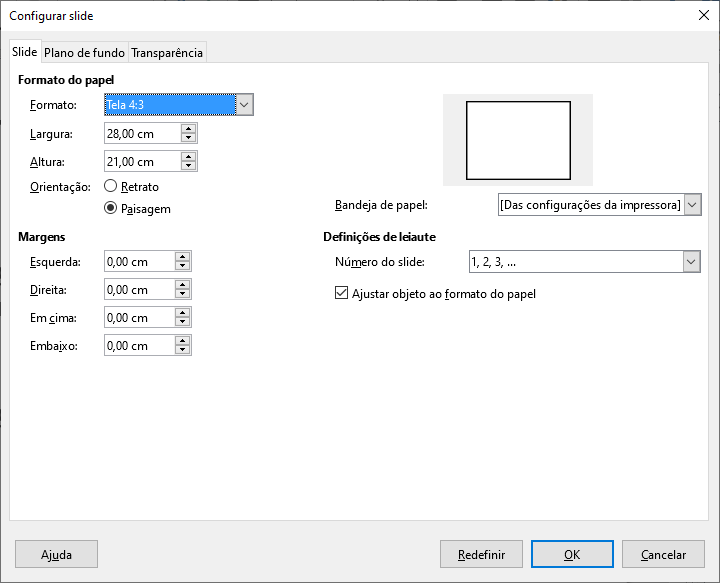
\includegraphics[width=0.65\linewidth]{Figuras/Ch05/fig16.3}
\end{frame}


\begin{frame}{Preparando uma apresentação}
	\begin{block}{Como fazer uma boa apresentação de slides?}
		\begin{itemize}
			\item Uma boa organização dos slides é crucial para uma apresentação interessante, mas apenas isto não basta.
			\item Dominar o conteúdo é imprescindível para que a apresentação seja bem organizada e bem passada para a plateia.
		\end{itemize}
	\end{block}
\end{frame}



\begin{frame}{Preparando uma apresentação}
	\begin{block}{Como fazer uma boa apresentação de slides?}
		As ideias devem estar encadeadas na \textbf{ordem lógica}:
		\begin{itemize}
			\item capa;
			\item apresentação pessoal (de acordo com a ocasião);
			\item introdução;
			\item desenvolvimento do tema;
			\item conclusão.
		\end{itemize}
	\end{block}

	%	\centering
	%	\includegraphics[width=0.7\linewidth]{Figuras/Ch05/fig}
\end{frame}



\begin{frame}{Preparando uma apresentação}
	\begin{block}{Como fazer uma boa apresentação de slides?}
		\begin{itemize}
			\item Listar apenas \textbf{tópicos}.
			\item Não expressar \textbf{ideias completas} e \textbf{conceitos longos} (apenas se realmente necessários).
			\item \textbf{Evitar acúmulo} de \textbf{caracteres} ou \textbf{ideias diferentes} no mesmo slide.
			\item Imagens devem ser \textbf{explicadas} pelo palestrante.
		\end{itemize}
	\end{block}

	%	\centering
	%	\includegraphics[width=0.7\linewidth]{Figuras/Ch05/fig}
\end{frame}



\begin{frame}{Preparando uma apresentação}
	\begin{block}{Como fazer uma boa apresentação de slides?}
		\begin{itemize}
			\item Usar plano de fundo e fonte \textbf{em contraste}.
			\item O plano de fundo deve \textbf{combinar} com o assunto que trata a apresentação (ou ser neutro).
			\item \textbf{Evitar} o uso de \textbf{cores vibrantes}.
			\item \textbf{evitar} o uso de fonte de \textbf{tamanho pequeno}.
			\item O foco é o \textbf{assunto} e \textbf{não} o que está \textbf{escrito} no slide.
			\item A plateia deve prestar \textbf{mais atenção} no que o \textbf{palestrante tem a dizer} sobre o assunto do que nos slides.
		\end{itemize}
	\end{block}

	%	\centering
	%	\includegraphics[width=0.7\linewidth]{Figuras/Ch05/fig}
\end{frame}



\begin{frame}{Preparando uma apresentação}
	\begin{block}{Como fazer uma boa apresentação de slides?}
		Uma boa apresentação serve \textbf{apenas} para \textbf{direcionar o raciocínio} e deve ser \textbf{ilustrada} com:
		\begin{itemize}
			\item gráficos;
			\item figuras;
			\item fluxogramas;
			\item vídeos;
			\item entre outros \textbf{elementos visuais}...
		\end{itemize}
	\end{block}

	%	\centering
	%	\includegraphics[width=0.7\linewidth]{Figuras/Ch05/fig}
\end{frame}


\begin{frame}{O que não fazer}
	\begin{block}{}
		\begin{itemize}
			\item Vamos observar quais \textbf{problemas} os slides a seguir têm?
		\end{itemize}
	\end{block}

	\centering
	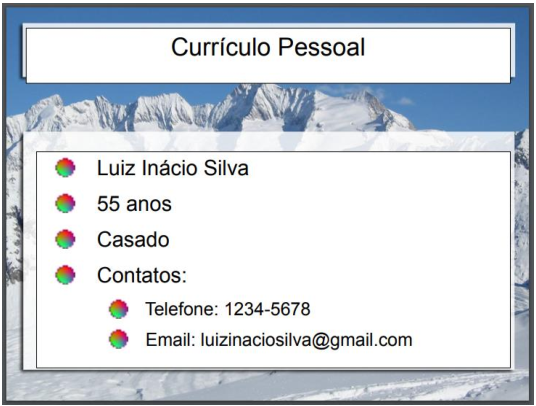
\includegraphics[width=0.7\linewidth]{Figuras/Ch05/fig17}
\end{frame}


\begin{frame}{O que não fazer}
	\centering
	
\includegraphics[width=0.7\linewidth]{Figuras/Ch05/fig18}
\end{frame}


\begin{frame}{O que não fazer}
	\centering
	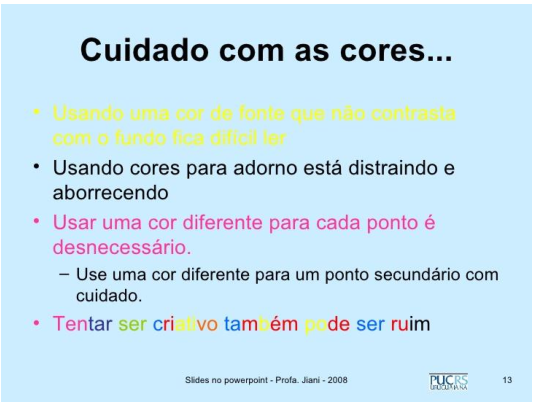
\includegraphics[width=0.7\linewidth]{Figuras/Ch05/fig19}
\end{frame}


\begin{frame}{O que não fazer}
	\centering
	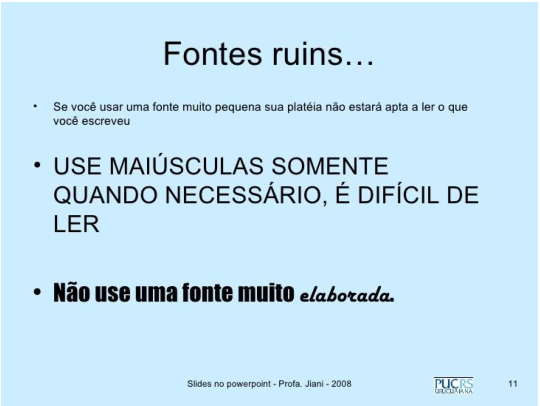
\includegraphics[width=0.7\linewidth]{Figuras/Ch05/fig20}
\end{frame}


\begin{frame}{O que não fazer}
	\centering
	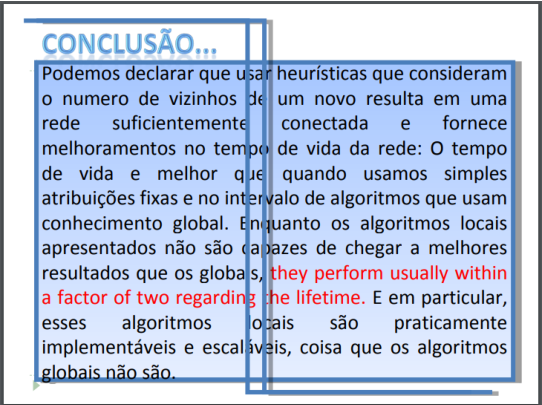
\includegraphics[width=0.7\linewidth]{Figuras/Ch05/fig21}
\end{frame}


\begin{frame}{Tipos de impressão de slides}
	\begin{block}{}
		\begin{itemize}
			\item Antes da impressão de slides, é necessário primeiramente definir a \textbf{utilidade} e o \textbf{tamanho adequado}.
			\item \textbf{Nem sempre} o ideal é imprimir \textbf{um por página}.
			\item Usar a impressão padrão pode \textbf{elevar o custo} e o \textbf{volume de papel}.
			\item Nas opções de impressão, pode-se escolher o \textbf{formato} da impressão:
			\begin{itemize}
				\item Menu Arquivo > Imprimir ou Ctrl + P. (Como no Writer)
			\end{itemize}
		\end{itemize}
	\end{block}

	%	\centering
	%	\includegraphics[width=0.7\linewidth]{Figuras/Ch05/fig}
\end{frame}


\begin{frame}{Tipos de impressão de slides}
%	\begin{block}{}
%		\begin{itemize}
%			\item Para imprimir um por página.
%		\end{itemize}
%	\end{block}

	\centering
	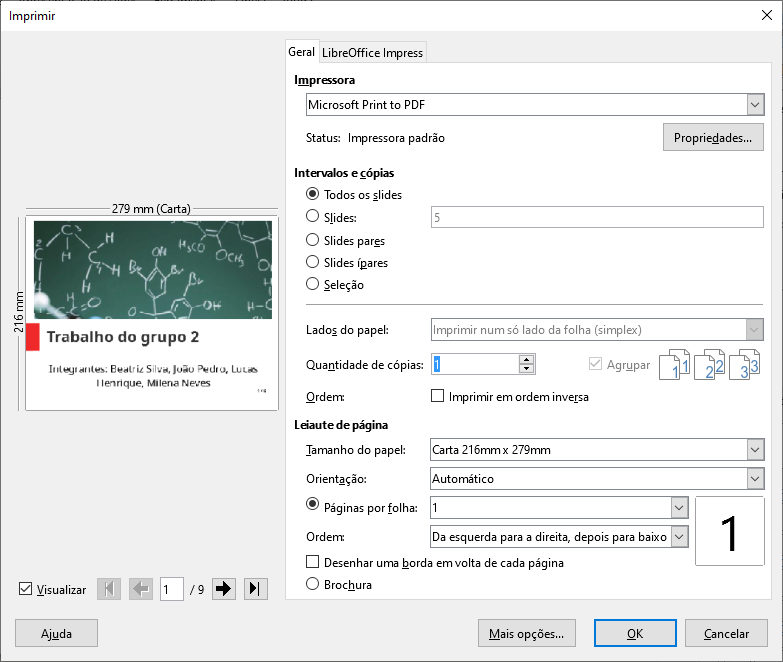
\includegraphics[width=0.75\linewidth]{Figuras/Ch05/fig22}
\end{frame}


\begin{frame}{Tipos de impressão de slides}
	\begin{block}{}
		\begin{itemize}
			\item Para imprimir folhetos.
		\end{itemize}
	\end{block}

	\centering
	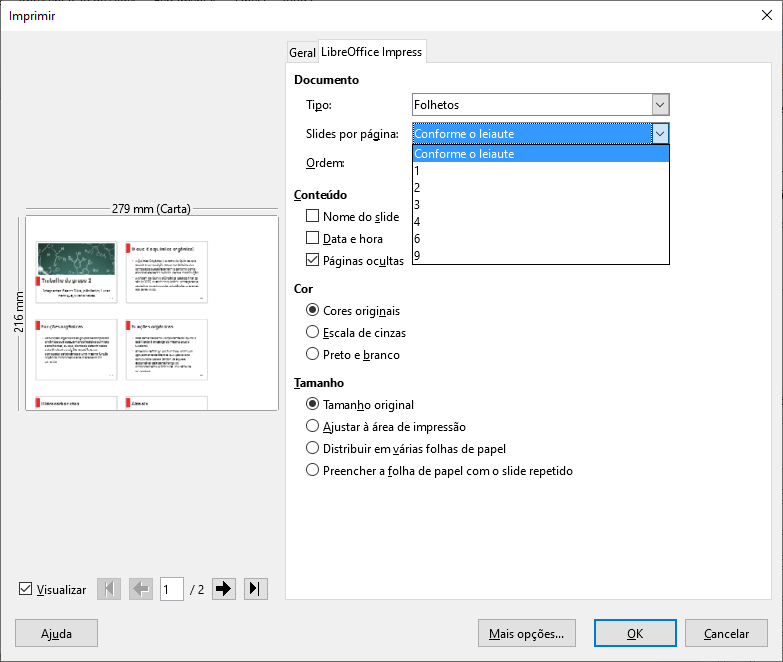
\includegraphics[width=0.65\linewidth]{Figuras/Ch05/fig23}
\end{frame}


%\begin{frame}{Atividade 1 --- Usar transições}
%	\begin{block}{}
%		\begin{itemize}
%			\item 
%			Fazer uma apresentação sobre você com as seguintes instruções:
%			Slide 1 → Layout de Título
%			Seu nome completo
%			Slide 2 → Layout de Título e Conteúdo
%			Título – Seu nome completo
%			Tópicos – Gostos e preferências → usar marcadores.
%			Slide 3 → Layout de Título e 2 Conteúdos
%			Título – Seu nome completo
%			Conteúdo 1 – Vida acadêmica (Onde você estudou), usando marcadores;
%			Conteúdo 2 – Inserir tabela – Tabela com informação de curso superior.
%		\end{itemize}
%	\end{block}
%	
%	\centering
%	\includegraphics[width=0.7\linewidth]{Figuras/Ch05/fig}
%\end{frame}


\section*{Exercícios}
\frame{
	\frametitle{Exercícios}
	\begin{block}{}
		01. Você tem vergonha de fazer apresentações? E se tivesse slides para te auxiliar, acha que ficaria mais fácil?
		
		\medskip
		
		02. Você já se imaginou apresentando algo em uma grande companhia ou na faculdade? O que você gostaria de apresentar?
		
		\medskip
		
		03. Monte uma apresentação sobre um assunto que te interessa, ou até sobre o que aprendeu até agora no curso técnico.
	\end{block}
}

\section*{Referências}

\frame{
	\frametitle{Referências e Exercícios Complementares}
	\begin{itemize}
		\item Introdução ao LibreOffice, \href{https://documentation.libreoffice.org/assets/Uploads/Documentation/pt-br/GS50/GS50-IntroducaoLO-5.0-ptbr.pdf}{Apostila de uso livre}.
	\end{itemize}
	%\centering{\alert{Página 36 - \textbf{1.6.1 até 1.6.5, 1.6.17 até 1.6.19}}} \\
	%	\centering{\alert{Lista de exercícios 01}}
}